\documentclass[11pt,a4paper]{article}

\usepackage[utf8]{inputenc}
\usepackage{amsmath}
\usepackage{amsfonts}
\usepackage{amssymb}
\usepackage{graphicx}
\usepackage{hyperref}
\usepackage{geometry}
\usepackage{booktabs}
\usepackage{caption}
\usepackage{subcaption}
\usepackage{float}
\usepackage{xcolor}

\geometry{margin=1in}

% Status callouts, built from xcolor alone so this file compiles with a base LaTeX
% installation. Both environments break across pages.
\definecolor{gapred}{rgb}{0.62,0.13,0.10}
\definecolor{okgreen}{rgb}{0.09,0.38,0.20}

\newenvironment{gapbox}[1]{%
  \par\medskip\noindent
  \textcolor{gapred}{\rule{\linewidth}{1.1pt}}\par\nobreak\vspace{2pt}%
  \noindent\textcolor{gapred}{\textbf{NOT YET DONE --- #1}}%
  \par\nobreak\vspace{3pt}%
  \begingroup\leftskip=1.2em\relax\small
}{%
  \par\endgroup\vspace{3pt}%
  \noindent\textcolor{gapred}{\rule{\linewidth}{0.5pt}}\par\medskip
}

\newenvironment{okbox}[1]{%
  \par\medskip\noindent
  \textcolor{okgreen}{\rule{\linewidth}{1.1pt}}\par\nobreak\vspace{2pt}%
  \noindent\textcolor{okgreen}{\textbf{VERIFIED --- #1}}%
  \par\nobreak\vspace{3pt}%
  \begingroup\leftskip=1.2em\relax\small
}{%
  \par\endgroup\vspace{3pt}%
  \noindent\textcolor{okgreen}{\rule{\linewidth}{0.5pt}}\par\medskip
}

\title{Thalamocortical Gating Project Documentation \\
\large Methodological and Theoretical Foundations}
\author{Thalamocortical Gating Project}
\date{Last verified 2026-08-26}

\begin{document}

\maketitle

\begin{abstract}
This document records the modelling architecture, experimental protocols and theoretical
foundations of the project. The project \emph{synthesises} two published models: the
dendritic disinhibitory gating circuit and Graupner--Brunel calcium plasticity of
Yang et al.\ (2016), and the cell-type-specific mediodorsal-thalamic (MD) projections of
Zhang et al.\ (2025). Throughout, we distinguish the \emph{intended} behaviour (the
project specification) from the \emph{verified} behaviour of the current code, and we
distinguish what is \emph{faithful} to the source papers from what is a \emph{novel
graft}. All parameter values quoted as ``Yang's'' have been checked against Yang 2016's
Methods (pp.~11--12); see Section~\ref{sec:provenance}. As of the last verification, the
central mechanism --- dendritic inhibition gating \emph{which} branch undergoes plasticity
--- is \textbf{demonstrated at the single-neuron level} (Section~\ref{sec:verification});
what remains is quantitative replication of Yang's figures and scaling to a network.
\end{abstract}

\section{Project Overview}
The goal is to model \textbf{pathway-specific gating} in the prefrontal cortex (PFC),
controlled by the mediodorsal thalamus (MD). By regulating local inhibitory interneurons
(VIP, SOM, PV), MD drive should control which dendritic branches of PFC pyramidal neurons
undergo calcium-based synaptic plasticity, enabling context-specific learning without
catastrophic forgetting. The single-neuron version of this mechanism now works
(Section~\ref{sec:verification}); the network-scale version and the full quantitative
replication of Yang do not yet exist (Sections~\ref{sec:bugs} and~\ref{sec:verification}).

\section{Relationship to the Source Papers}
\label{sec:papers}
The project's stated arc is \emph{replicate Yang 2016 $\rightarrow$ extend to Zhang 2025
$\rightarrow$ build a scalable network}. Because the two papers are different classes of
model, it is essential to be precise about what is inherited and what is not
(Table \ref{tab:papers}).

\begin{table}[H]
    \centering
    \small
    \begin{tabular}{@{}lp{5.0cm}p{5.0cm}@{}}
    \toprule
     & \textbf{Yang et al.\ 2016} (Nat.\ Commun.\ 7:12815) & \textbf{Zhang et al.\ 2025} (Nat.\ Commun.\ 16:2640) \\ \midrule
    Model class      & Spiking / reduced-compartment & Rate-based RNN, ML-trained (backprop-through-time) \\
    Dendrites        & Yes --- the mechanism         & None \\
    Plasticity       & Graupner--Brunel calcium      & None (trained weights) \\
    MD thalamus      & Absent (abstract control)     & Reciprocal PFC$\leftrightarrow$MD loop; MD$\rightarrow$Exc, MD$\rightarrow$PV, MD$\rightarrow$VIP \\
    Headline result  & Branch-specific dendritic gating & MD aids working memory / switching under low cue SNR \\ \bottomrule
    \end{tabular}
    \caption{The two source models are not the same kind of object. The project builds on
    Yang's framework and borrows only Zhang's cell-type wiring labels.}
    \label{tab:papers}
\end{table}

\paragraph{What is genuinely inherited.}
From Yang 2016: the reduced multi-compartment pyramidal cell, the VIP$\rightarrow$SOM
$\rightarrow$dendrite disinhibition and PV$\rightarrow$soma motifs, GABA$_A$ shunting,
the NMDA plateau nonlinearity, the Graupner--Brunel plasticity rule, and --- exactly ---
the dendritic I/O transfer function (Eq.~20--22) and all fitted plasticity constants
(Section \ref{sec:provenance}). From Zhang 2025: the two cell-type-specific MD
projections, MD$\rightarrow$PV (their MD$^{\text{GRIK4}}$ pathway) and MD$\rightarrow$VIP
(their MD$^{\text{DRD2}}$ disinhibitory pathway). The marker$\rightarrow$target pairing is
verified against Zhang: \textbf{GRIK4 (kainate receptor) $\rightarrow$ PV} and
\textbf{DRD2 (dopamine D2) $\rightarrow$ VIP}, not swapped. One wording caveat: Zhang
frames MD$^{\text{GRIK4}}\rightarrow$PV as \emph{feedforward inhibition / prefrontal-noise
suppression}; ``gain control'' in that paper denotes the VIP--SOM motif and corticothalamic
modulation, not MD$\rightarrow$PV directly. Labelling MD$\rightarrow$PV ``gain control'' is
a defensible paraphrase but not the paper's literal attribution.

\paragraph{What is \emph{not} done.}
This is a \textbf{novel synthesis, not a replication of either paper.}
\begin{itemize}
    \item Yang's gating is reproduced \emph{at the single-neuron level} (Section
      \ref{sec:verification}), but not as Yang's quantitative figures (Fig.~2c I/O,
      Fig.~7b LTP-threshold shift, Fig.~7d--e) and not at network scale.
    \item It does not reproduce or extend Zhang's model. Zhang is a trained rate RNN
      performing a cognitive task; none of the task, psychometric curves, working-memory
      delay, attractor analysis, or the SOM$\rightarrow$Exc-sparsity E/I result is
      implemented. Only Zhang's \emph{wiring labels} are used, and even then the
      reciprocal PFC$\leftrightarrow$MD loop and the MD$\rightarrow$excitatory projection
      are omitted --- MD here is a bare external \texttt{PoissonGroup}.
    \item The scalable-network stage is essentially unstarted: Yang's network is
      $\sim$3{,}000 pyramidal $+$ 160 SOM $+$ 140 VIP $+$ 200 PV neurons with $\sim$30
      dendrites each; Model A here is 1 pyramidal soma, 2 dendrites, 20 of each
      interneuron.
\end{itemize}

\section{Status of the Two Former Blocking Bugs}
\label{sec:bugs}
Both were calibration/formulation errors against Yang 2016's own Methods. \textbf{Both are
now fixed in Model A} (the Brian 2 model), which is what makes Phase-1 gating pass. They
remain in the two NumPy figure models (B, C), which are frozen as illustrative sketches.

\begin{okbox}{Bug 1 (drive too weak) --- fixed in Model A}
Yang sets the maximum excitatory conductance per dendrite to $g_{E,\max}=25$~nS, with
half-activation $g_{1/2}=\beta_g(g_{L,D}+g_{\text{inh}})=5.56\,(4+g_{\text{inh}})$~nS
(Eqs.~21--22; the ``4'' is the dendritic leak $g_{L,D}=4.0$~nS). A disinhibited branch
($g_{\text{inh}}\approx2$~nS) has $g_{1/2}\approx33$~nS and, driven near plateau,
\emph{activates}; an inhibited branch ($g_{\text{inh}}\approx35$~nS) has
$g_{1/2}\approx217$~nS and stays at rest. The Phase-1 experiment drives the pathway at
$80$~Hz with Yang's \emph{in-vivo} dendrite--soma coupling $g_c=0.8$~nS
(\texttt{gEachCouple\_pyr\_vivo}; the older experiments used $4.0$~nS, which drove the soma
to $\sim$200~Hz). The NumPy figure models still use the old sub-threshold drive and remain
inert.
\end{okbox}

\begin{okbox}{Bug 2 (calcium model not Yang's) --- fixed in Model A}
Yang's dendritic calcium has \emph{two} components (Methods p.~11):
\begin{itemize}
    \item \textbf{NMDA calcium}, a leaky integral of the NMDA current (Eq.~13):
      $\tau_{\text{Ca}}\,d[\text{Ca}]_{\text{NMDA}}/dt = -[\text{Ca}]_{\text{NMDA}}
      + \kappa_{\text{NMDA}}\,I_{\text{NMDA}}$, where $\kappa_{\text{NMDA}}=0.371$ (unit
      \emph{per pA}) scales a \emph{current}; under a plateau this accumulates past
      $\theta_p=2.78$ and yields LTP.
    \item \textbf{VGCC calcium}, per-spike bumps from back-propagating APs (Eq.~14), a sum
      of bi-exponential transients with per-spike peak $\kappa_{\text{VGCC}}=0.957$.
\end{itemize}
Model A now implements exactly this: \texttt{equations.py} integrates the NMDA-current
calcium ($\kappa\cdot g_{\text{NMDA}}\,s_{\text{nmda}}\,\text{mg}\,(v_E-V)$, Eq.~13) and
reads the branch's bAP transient \texttt{bAPCa} (Eq.~14) as the postsynaptic component.
Models B and C instead treat $\kappa_{\text{NMDA}}$ as a fixed \emph{per-spike} jump,
capping single-pairing calcium at $0.371+0.957=1.328<\theta_p$, so \textbf{LTP stays
structurally impossible in B and C}. (Yang's rule was \emph{fit} to spike pairings but
\emph{deployed} with Poisson rate trains at a fixed 10~Hz post rate, so a single pair
failing to reach $\theta_p$ is expected, not a defect.)
\end{okbox}

\section{Provenance of the Constants}
\label{sec:provenance}
An earlier note in this repository claimed these constants were unsourced --- it cited
\texttt{data/parameters.txt} / \texttt{data/equations.txt} files that \textbf{never existed
in any commit}. That was a documentation gap, not a values problem: \textbf{every constant
is Yang 2016's published value}, verified against the paper (Methods pp.~11--12).

\begin{table}[H]
    \centering
    \small
    \begin{tabular}{@{}lll@{}}
    \toprule
    \textbf{Constant (code)} & \textbf{Yang 2016 value} & \textbf{Location} \\ \midrule
    \texttt{theta\_p}=2.78 & $\theta_p=2.78$ & Methods p.~12 \\
    \texttt{theta\_d}=1.0 & $\theta_d=1$ (fixed, from Graupner--Brunel ref.~36) & Methods p.~12 \\
    \texttt{gamma\_d}=39.949 / \texttt{gamma\_p}=177.552 & $\gamma_d=39.9$ / $\gamma_p=177.6$ & Methods p.~12 \\
    \texttt{tau}=346.36~s & $\tau_\rho=346.36$~s (the $\rho$/weight time constant) & Methods p.~12 \\
    \texttt{sigma}=3.35 & $\sigma=3.35$ (from ref.~36) & Methods p.~12 \\
    $\kappa_{\text{NMDA}}$=0.371 (NumPy \texttt{C\_NMDA}) & $\kappa_{\text{NMDA}}=0.371$ & Methods p.~12, Eq.~13 \\
    $\kappa_{\text{VGCC}}$=0.957 (NumPy \texttt{C\_BAP}) & $\kappa_{\text{VGCC}}=0.957$ & Methods p.~12, Eq.~14 \\
    \bottomrule
    \end{tabular}
    \caption{The dendritic I/O function \texttt{dend\_IO} likewise reproduces Yang's
    Eq.~20--22 exactly ($\beta_g$=5.56, $k$=9.64~nS, $\gamma$=6.54~nS, $V_0$=0.78~mV;
    Methods p.~11), and $g_{E,\max}=25$~nS, $g_{L,D}=4.0$~nS match Yang.}
\end{table}

Three distinctions the papers make and the earlier docs blurred:
\begin{itemize}
    \item \texttt{tau}$=346.36$~s is the $\rho$ (synaptic-weight) time constant, \emph{not}
      a calcium time constant. Yang's calcium decays with $\tau_{\text{Ca,decay}}=30$~ms
      (\texttt{tau\_Ca\_NMDA}$=30$~ms here).
    \item $\kappa_{\text{NMDA}}$ (unit \emph{per pA}) scales the NMDA \emph{current} in a
      leaky integral (Eq.~13); $\kappa_{\text{VGCC}}$ is the \emph{per-postspike bump peak}
      (Eq.~14). Treating either as a symmetric per-spike jump --- as Models B/C do --- is
      Bug~2.
    \item In vivo, Yang scales both down: $\hat\kappa_{\text{NMDA}}=0.75\,\kappa_{\text{NMDA}}
      =0.278$, $\hat\kappa_{\text{VGCC}}=0.2\,\kappa_{\text{VGCC}}=0.191$. Model A's
      calibrated \texttt{kappa\_Ca\_NMDA}$=0.26$~/pA sits close to Yang's in-vivo
      $0.278$~/pA --- a near-coincidence reached by Phase-1 calibration, not a cited value.
\end{itemize}

\section{Three Implementations}
\label{sec:three}
This project contains \textbf{three independent implementations}, not one. They agree on
parameter values by convention but share no code, and each figure comes from exactly one
of them (Table \ref{tab:models}).

\begin{table}[H]
    \centering
    \small
    \begin{tabular}{@{}llp{6.2cm}@{}}
    \toprule
    \textbf{Model} & \textbf{Files} & \textbf{Role} \\ \midrule
    \textbf{A.} Brian 2 spiking net
      & \texttt{src/v2/}, \texttt{experiments/}
      & Full spiking circuit; MD as \texttt{PoissonGroup}; native Graupner--Brunel
        synapses with Yang's Eq.~13/14 calcium. The canonical model, and the only one in
        which plasticity is active. Source of Figure \ref{fig:architecture} and of the
        Phase-1 gating result. \\ \addlinespace
    \textbf{B.} Phenomenological
      & \texttt{main\_gating\_figures.py}
      & Pure NumPy; hardcoded dendritic inhibition. Source of Figures 1--4. Plasticity
        inert (Bugs 1 \& 2 remain here). \\ \addlinespace
    \textbf{C.} Emergent mechanistic
      & \texttt{emergent\_gating\_mechanistic\_model.py}
      & Pure NumPy; inhibition emerges from noisy interneuron rates. Source of the
        mechanistic figures. Plasticity inert (Bugs 1 \& 2 remain here). \\ \bottomrule
    \end{tabular}
    \caption{The three implementations. Models B and C do not import \texttt{src/v2/}.
    Both also replace Graupner--Brunel's bistable $\rho$ dynamics with a \emph{monostable}
    relaxation toward $\bar\rho$ at rate $\eta_\rho=0.08$, so their ``bistable'' figure
    captions are not supported by the code.}
    \label{tab:models}
\end{table}

\section{The MD Thalamus as a Poisson Group (Model A)}
\label{sec:poisson}
In Model A the MD thalamus is a \textbf{Poisson spiking group} (\texttt{n\_md}$=50$ relay
cells), biologically motivated by the largely Poisson firing of thalamic relay neurons. It
projects with different probabilities and weights to different interneuron types:
\begin{itemize}
    \item \textbf{MD $\rightarrow$ PV:} $p=0.5$, $g_{\text{AMPA}}=0.12$~nS (feedforward
      somatic inhibition / noise suppression, Zhang's GRIK4 pathway).
    \item \textbf{MD $\rightarrow$ VIP:} $p=0.3$, $g_{\text{AMPA}}=0.5$~nS
      (context-selective disinhibition, Zhang's DRD2 pathway).
\end{itemize}

The total drive onto a postsynaptic cell scales as $p\cdot n_{\text{md}}\cdot g$:
\begin{align}
    \text{PV:}\quad  &0.5 \times 50 \times 0.12\,\text{nS} = 3.0\,\text{nS}, \\
    \text{VIP:}\quad &0.3 \times 50 \times 0.5\,\text{nS}\phantom{2} = 7.5\,\text{nS}.
\end{align}
So MD drive onto VIP is in fact $2.5\times$ stronger in aggregate; the selectivity
distinction rests on the sparser, stronger VIP connectivity, not on total drive.
\emph{Note:} unlike Zhang 2025, this MD group has no PFC$\rightarrow$MD feedback and no
MD$\rightarrow$excitatory projection.

\begin{figure}[H]
    \centering
    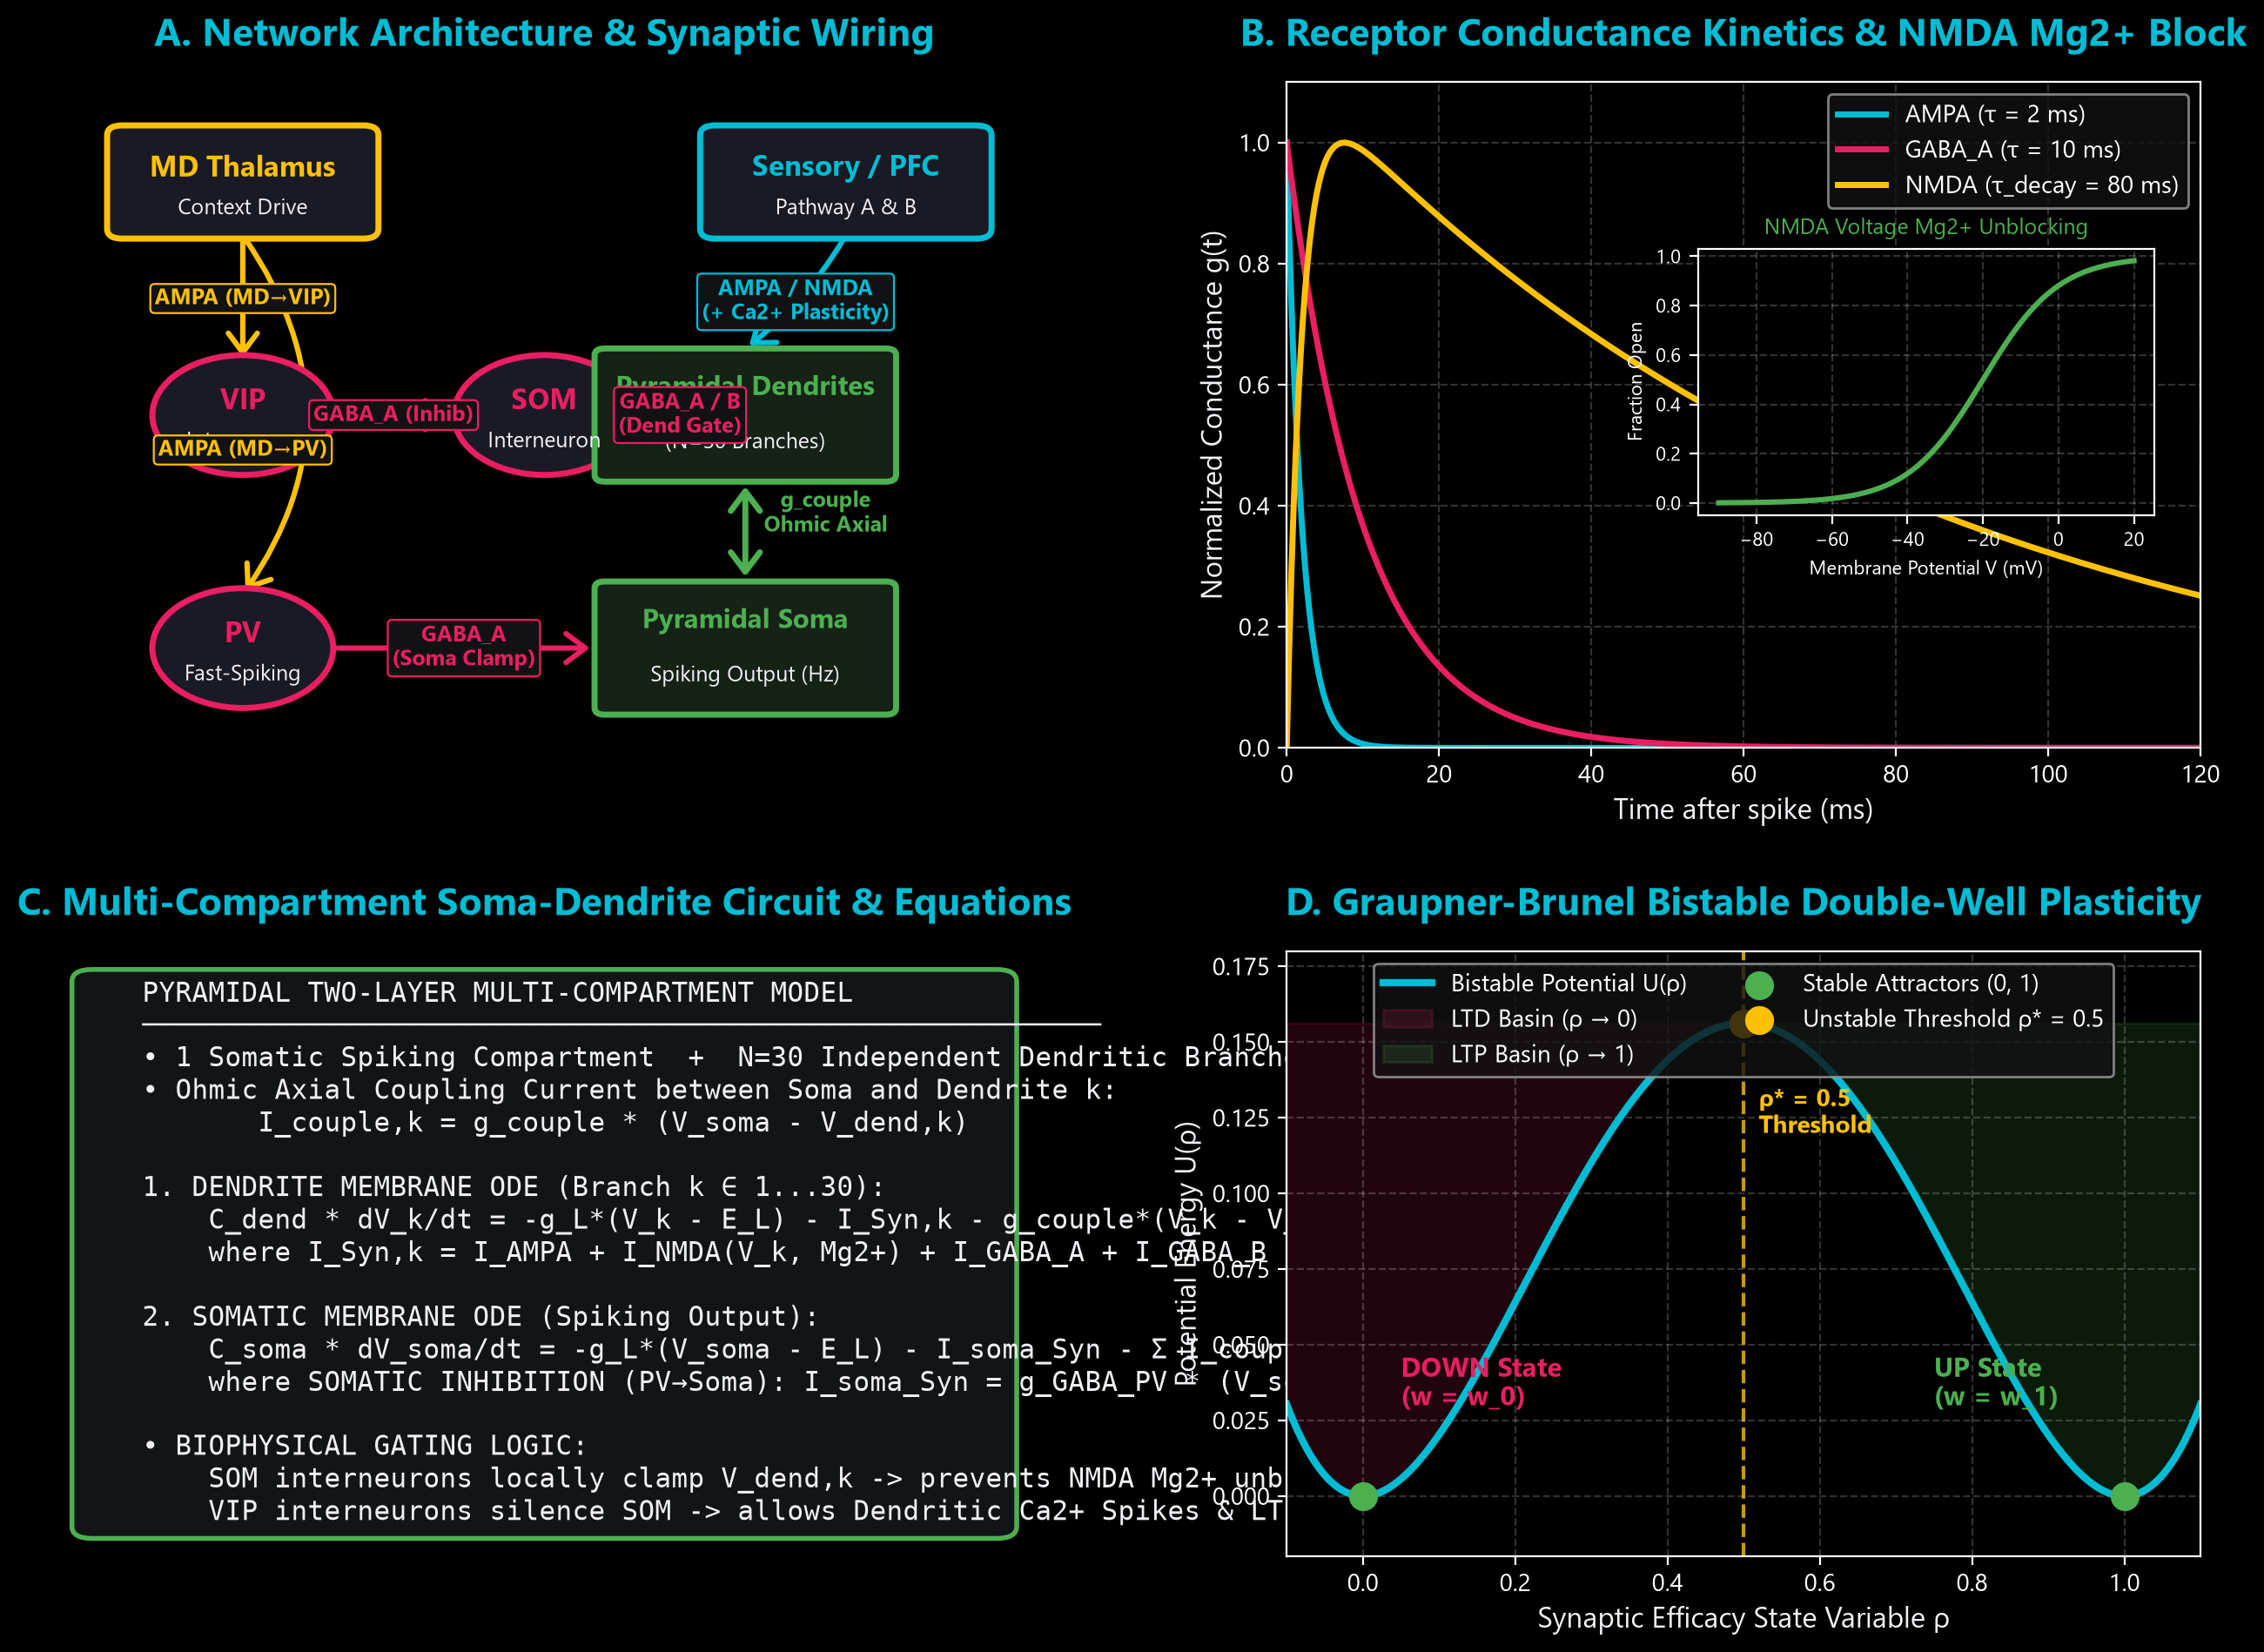
\includegraphics[width=\textwidth]{figures/network_synaptic_architecture.png}
    \caption{Network architecture and synaptic wiring. Generated by
    \texttt{experiments/generate\_network\_synapse\_figure.py}.}
    \label{fig:architecture}
\end{figure}

\begin{gapbox}{Figure \ref{fig:architecture} is hand-drawn, not introspected}
\texttt{generate\_network\_synapse\_figure.py} hardcodes every annotation, so the diagram
can drift from the code. It states $N=30$ dendritic branches (every runnable script uses
\textbf{2}) and mixes Model C's parameters with Model A's as though they described one
model. For an accurate, live snapshot use \texttt{print\_network\_summary.py}, which
builds the network and reads \texttt{len(group)} / \texttt{len(synapses)} directly.
\end{gapbox}

\section{Circuit Scale as Implemented (Model A)}
All values from \texttt{src/v2/parameters.py} as used by
\texttt{experiments/demo\_v2\_zhang2025.py}.

\begin{table}[H]
    \centering
    \small
    \begin{tabular}{@{}lll@{}}
    \toprule
    \textbf{Population} & \textbf{Size} & \textbf{Parameter} \\ \midrule
    Pyramidal soma                & 1           & \texttt{num\_Soma} \\
    Dendritic branches            & \textbf{2}  & \texttt{num\_DendEach} (per-script override; default 10 = Yang's reduced-model compartment count) \\
    MD thalamus (\texttt{PoissonGroup}) & 50    & \texttt{n\_md} \\
    PV / SOM / VIP interneurons   & 20 each     & \texttt{n\_pv}, \texttt{n\_som\_spike}, \texttt{n\_vip\_spike} \\
    Cortical pathway input        & 30 @ 80 Hz  & literal per script \\ \bottomrule
    \end{tabular}
    \caption{Implemented population sizes. Compare Yang's $\sim$3{,}000 pyramidal / 160
    SOM / 140 VIP / 200 PV / $\sim$30 dendrites: this is a single-neuron reduction, not a
    network. (Yang's \emph{reduced spiking} model in his Figs.~2 and~7 uses 10 dendritic
    compartments, which is the origin of the \texttt{num\_DendEach}=10 default.)}
\end{table}

SOM cells receive \textbf{no synaptic excitation}; their baseline comes from a bias
current \texttt{iBaseline\_som} ($22$~pA $\rightarrow$ $\sim$36--40~Hz measured). Two
divergences from Yang 2016, verified against the paper, are worth stating as divergences
rather than quirks:
\begin{itemize}
    \item \textbf{SOM baseline rate.} Yang 2016 runs SOM at $\sim$\textbf{10}~Hz
      (``SOM neurons receive 150~pA input current \dots baseline firing $\sim$10~Hz'',
      Methods p.~11); this project runs $\sim$4$\times$ higher. A high interneuron/somatic
      rate is what drove the historical bAP-swamping problem.
    \item \textbf{Missing SOM $\rightarrow$ PV synapse.} Yang 2016 \emph{includes}
      SOM$\rightarrow$PV inhibition (connection probability $P_{\text{SOM--PV}}=0.8$, used
      in his Fig.~6). This project defines \texttt{gGABA\_pv} for such a synapse but never
      wires it, so the \texttt{iGABA} term in \texttt{eqs\_pv} is always zero. It is an
      unfinished Yang connection, not an intentional simplification.
\end{itemize}

\section{The Two Figure-Generating Models}

\subsection{B. The Phenomenological Model}
\textit{Proof-of-concept of Yang et al.\ (2016).} It uses \textbf{hardcoded} inhibition
levels rather than simulating interneurons: the ``disinhibited''/``inhibited'' branches
are assigned fixed values ($2.0$ and $35.0$), scaled by \texttt{g\_inh = 0.8*inh} to
$1.6$~nS and $28.0$~nS. The model is \textbf{not deterministic}: it draws Poisson pathway
rates and applies Gaussian $\rho$ noise and the accelerated $\eta_\rho=0.08$ update.

\begin{itemize}
    \item \textbf{Figures 1--3} plot continuous-time relations (STDP curve, dendritic I/O
      sigmoid, weight-vs-rate). Figure 3 is a hand-calibrated surrogate
      (\texttt{\_weight\_change\_from\_ca} is, by its own docstring, ``a simplified
      steady-state version''), with invented lumped constants and a $\times50$ scale
      factor; its NMDA driving-force term is identically zero across the plotted range.
    \item \textbf{Figure 4} is a 300-trial branch-learning simulation --- currently a
      noise-driven random walk (Bugs 1 \& 2 remain in this NumPy model).
\end{itemize}

\begin{figure}[H]
    \centering
    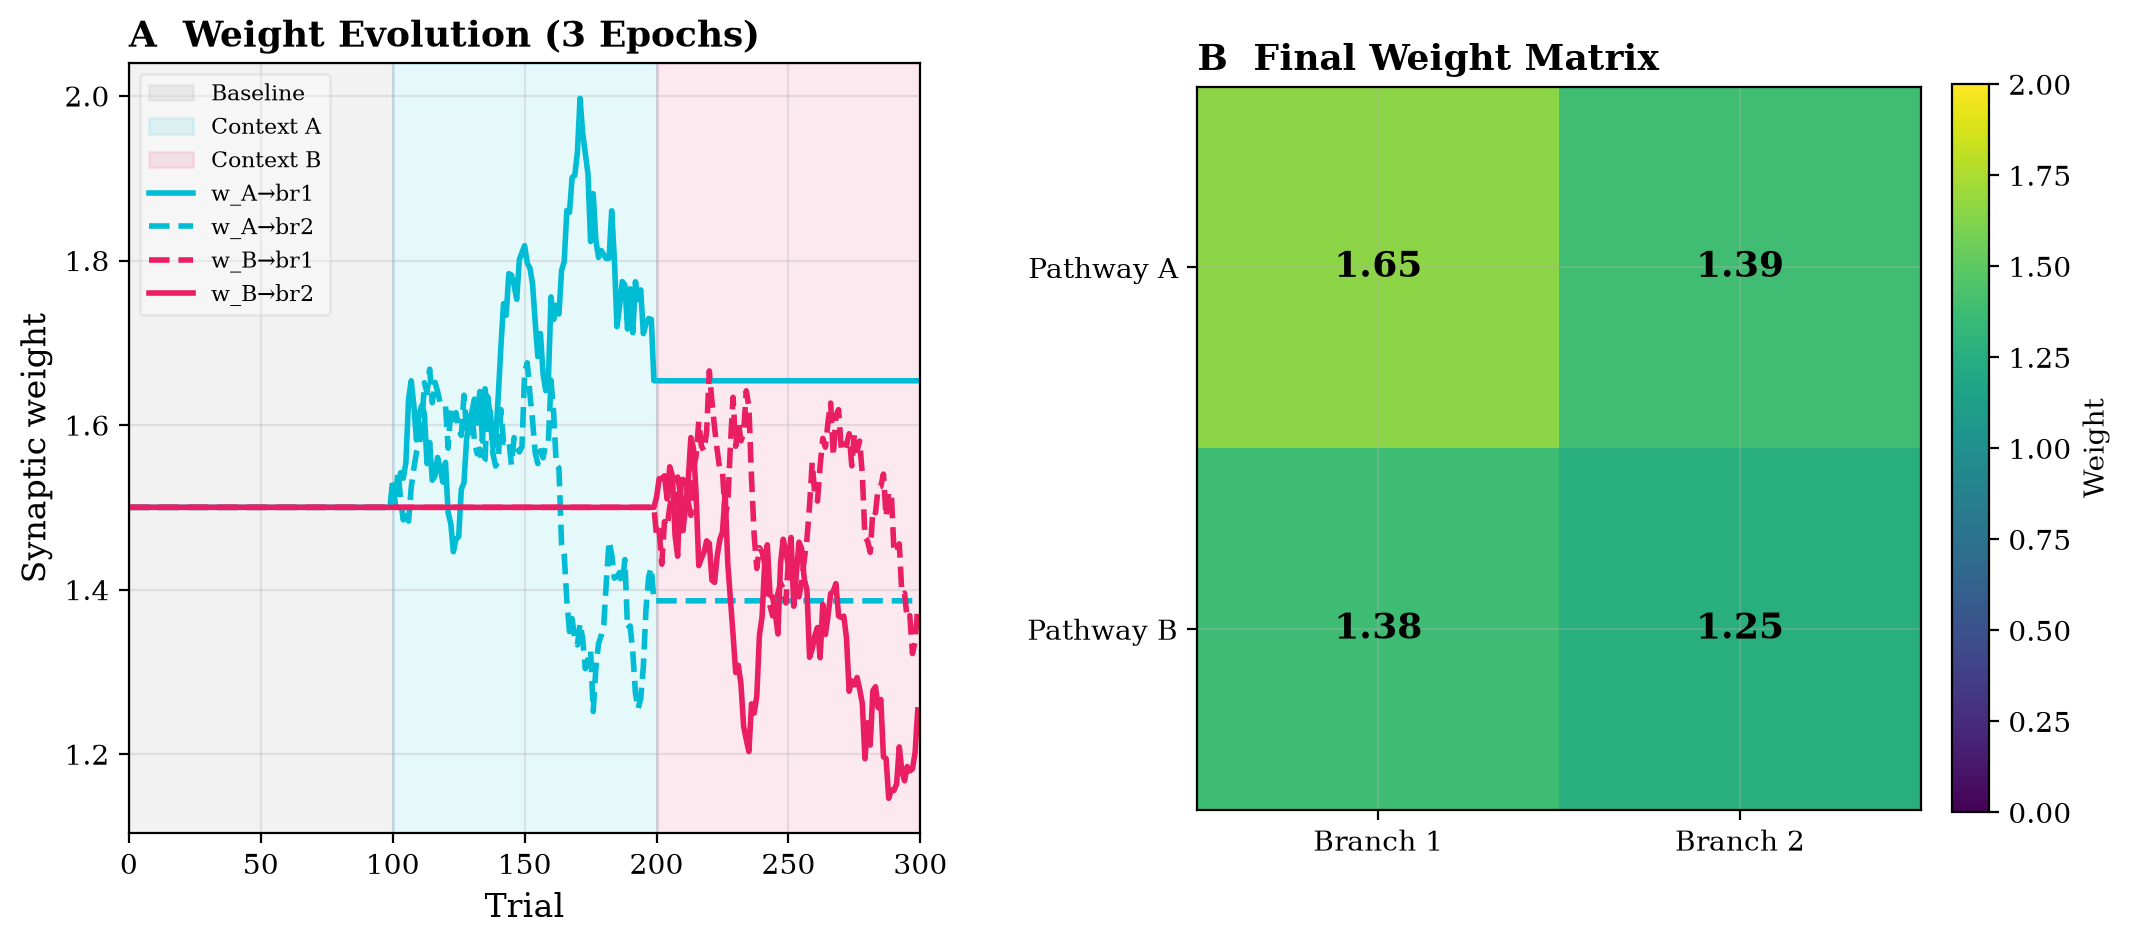
\includegraphics[width=0.85\textwidth]{figures/phenomenological/fig4_branch_specific_learning.png}
    \caption{Phenomenological branch-learning figure (hardcoded inhibition 1.6 / 28.0~nS).
    Does not currently show branch-specific learning --- see the box below.}
    \label{fig:phenom_learning}
\end{figure}

\subsection{C. The Emergent Mechanistic Model}
\textit{Fully stochastic sketch.} Inhibition emerges from a rate-based circuit:
$r_{\text{SOM}}=\max(0,\,40-1.5\,r_{\text{VIP}})$~Hz, branch conductance
$0.875\ \text{nS/Hz}\times r_{\text{SOM}}$. Noise sources: Poisson MD spike counts;
interneuron-rate variability (\texttt{CV\_RATE}$=0.20$, applied as $\sigma=0.20\,r$, i.e.\
\emph{linear} in rate, contrary to the module docstring's $\sqrt{\ }$ claim); vesicle noise
(\texttt{CV\_CA}$=0.30$); and $\rho$-update noise ($\sigma_\rho=0.04$) with the accelerated
$\eta_\rho=0.08$ in place of $\tau_\rho$.

\begin{figure}[H]
    \centering
    \begin{subfigure}[b]{0.48\textwidth}
        \centering
        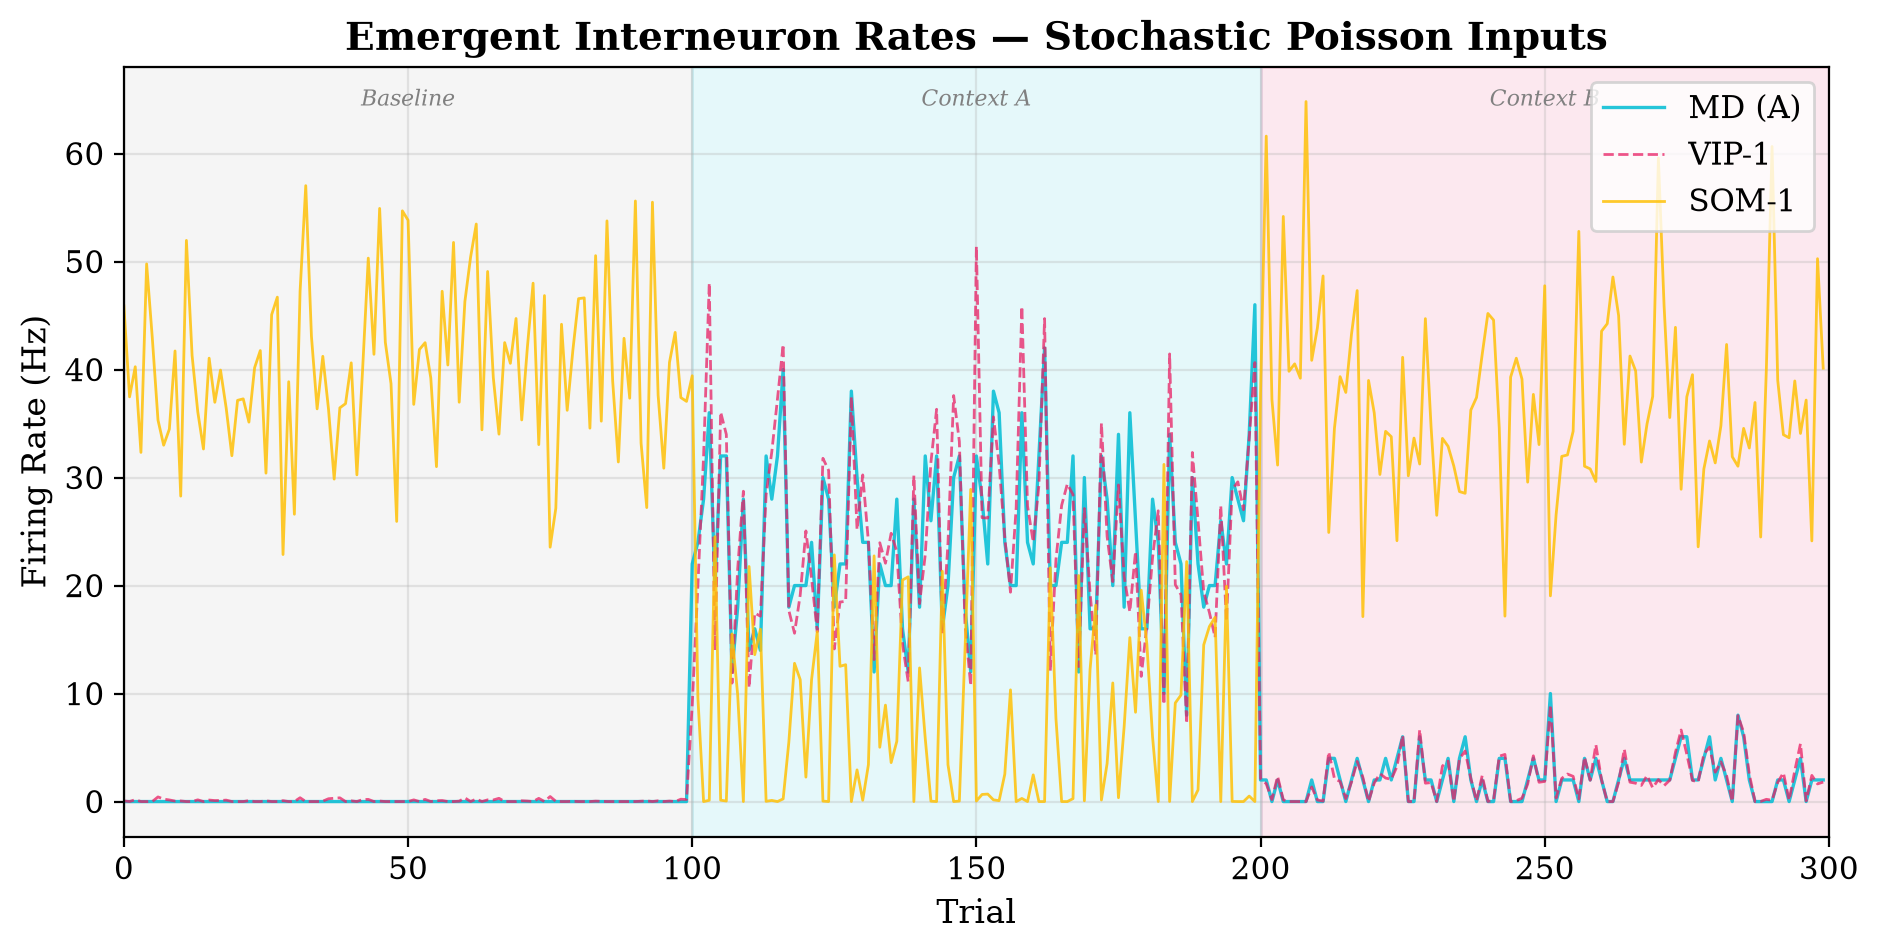
\includegraphics[width=\textwidth]{figures/mechanistic/fig_emergent_rates.png}
        \caption{Stochastic interneuron firing rates}
    \end{subfigure}
    \hfill
    \begin{subfigure}[b]{0.48\textwidth}
        \centering
        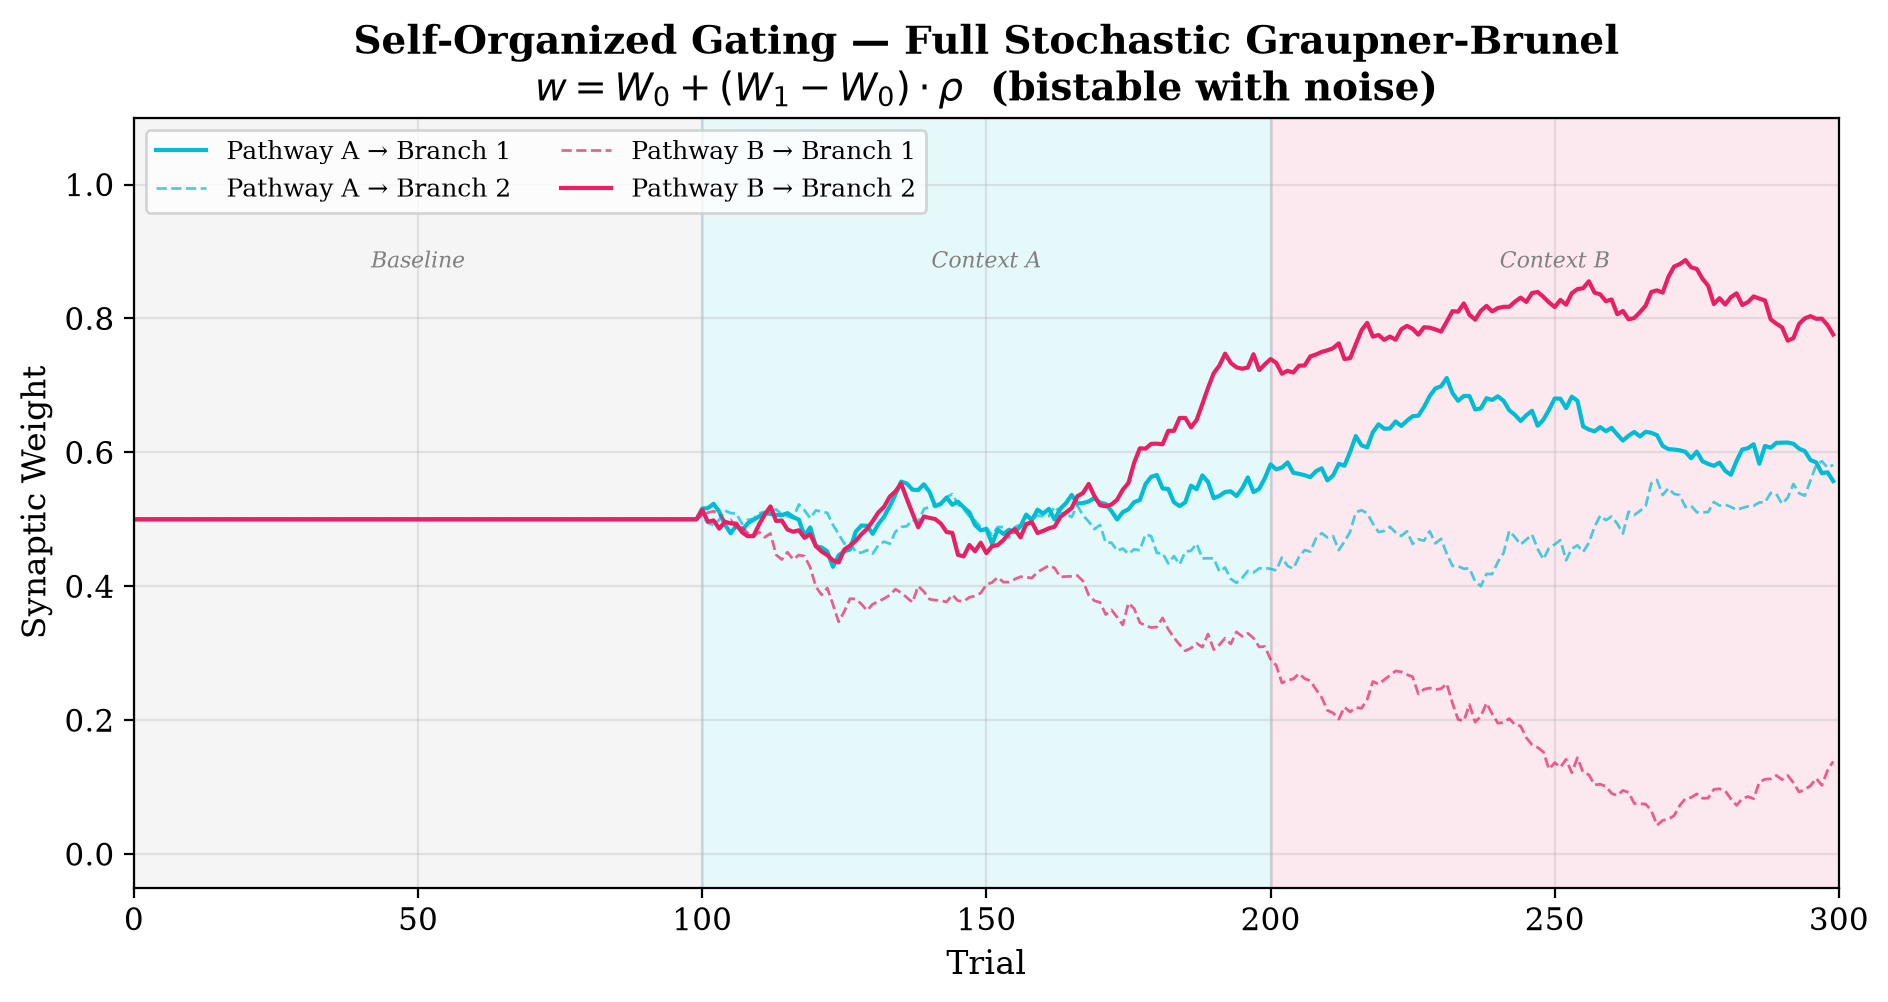
\includegraphics[width=\textwidth]{figures/mechanistic/fig_self_organized_branching.png}
        \caption{Weight trajectories under emergent inhibition}
    \end{subfigure}
    \caption{Output from the emergent mechanistic model. Panel (a) --- the interneuron
    rates doing their jobs --- is verified. Panel (b) does \textbf{not} show
    branch-specific learning; see the box below.}
    \label{fig:mechanistic_output}
\end{figure}

\begin{gapbox}{Plasticity is inert in both NumPy figure models (B and C)}
In B and C every Graupner--Brunel update falls to the calcium-inactive branch (peak calcium
$\approx0.02$ against $\theta_D=1.0$). At their operating point the dendrite sits at
$-68.9$~mV (disinhibited) vs $-69.1$~mV (inhibited) --- a $0.2$~mV difference --- so
Figures \ref{fig:phenom_learning} and \ref{fig:mechanistic_output}(b) are unbiased random
walks driven only by $\sigma_\rho$. Both bugs (sub-threshold drive; per-spike vs.\
integrated calcium) are fixed only in Model A, not in these NumPy sketches, which are kept
as illustrations. Porting the fixes to B/C would change every figure and is left undone
deliberately.
\end{gapbox}

\section{Experimental Protocol: The 3-Epoch Paradigm}
A continuous \textbf{300-trial} simulation (500~ms/trial) in three epochs, \textbf{Model C
only}: Baseline (0--99, both channels silent), Context~A (100--199, 25~Hz to VIP-1, 2~Hz
floor to VIP-2), Context~B (200--299, mirror image). The 2~Hz floor on the non-preferred
channel is deliberate and matters for the selectivity indices (Section \ref{sec:gs}).

\begin{gapbox}{This protocol is absent from the Brian 2 model}
\texttt{demo\_v2\_zhang2025.py} switches \emph{global} MD drive ($5\rightarrow40$~Hz) and
labels those levels ``Context A/B''; there are no separate VIP-1/VIP-2 channels, no
branch-selective targeting, and no baseline epoch. \texttt{sweep\_phase\_diagram.py} runs
a single fixed context at $40$~Hz. Porting the paradigm to Model A remains outstanding.
\end{gapbox}

\section{Gating Selectivity (Model C)}
\label{sec:gs}
$GS=(r_{\text{pref}}-r_{\text{non-pref}})/(r_{\text{pref}}+r_{\text{non-pref}})$.
Measured (seed 42): \textbf{VIP $=0.84$} (selective), \textbf{SOM $=-0.66$}
(anti-selective, the disinhibition signature), \textbf{PV $=-0.02$} (non-selective,
consistent with feedforward gain control). The departure of $GS_{\text{VIP}}$ from unity is
explained mostly by the 2~Hz background floor ($\tfrac{25-2}{25+2}=0.85$), not by Poisson
noise. These indices describe the \emph{interneuron rates}, not synaptic learning (which is
inert in Model C).

\begin{figure}[H]
    \centering
    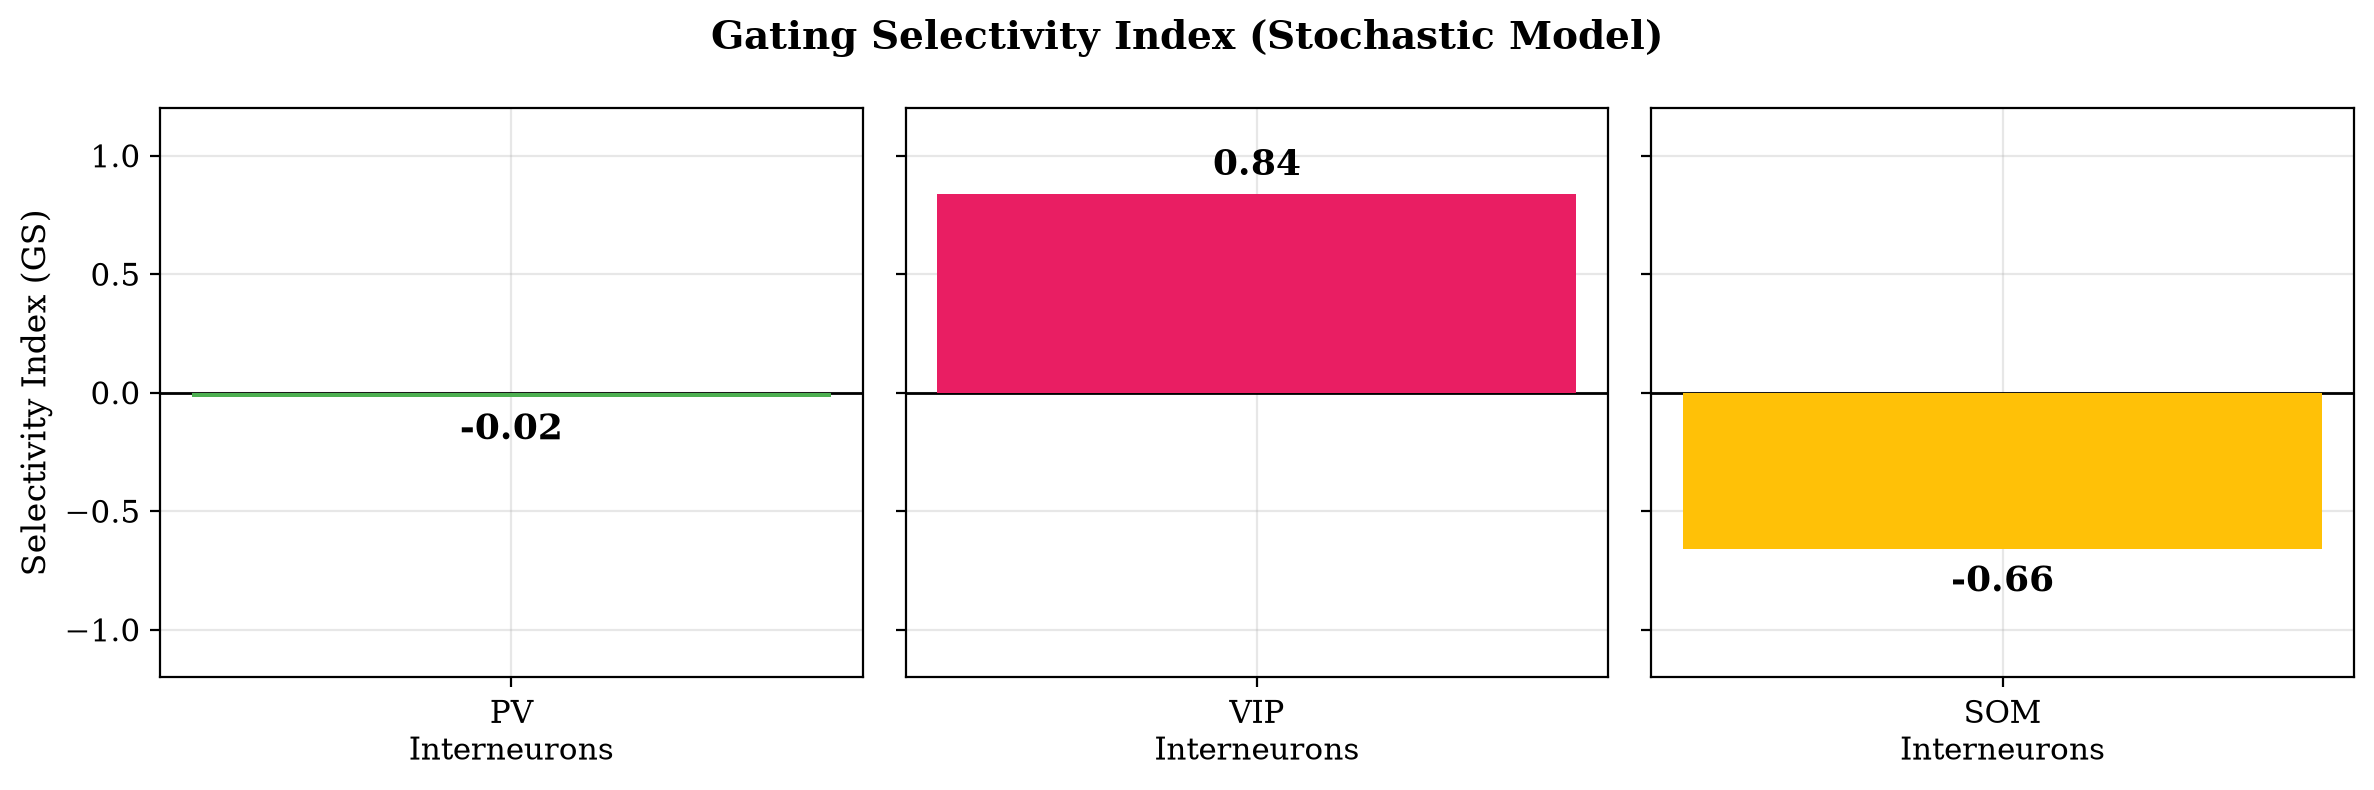
\includegraphics[width=0.75\textwidth]{figures/mechanistic/fig_gating_selectivity.png}
    \caption{Gating Selectivity indices for the three interneuron classes.}
    \label{fig:gs_scores}
\end{figure}

\section{Verification Status}
\label{sec:verification}
Everything below was established by executing the code.

\begin{okbox}{Verified working}
\begin{itemize}
    \item \textbf{Single-neuron branch-specific gating (Model A, Phase 1).}
      \texttt{experiments/phase1\_single\_neuron\_gating.py} at Yang's 10~Hz post rate,
      80~Hz pathway drive, $g_c=0.8$~nS coupling: the disinhibited (free) branch
      potentiates ($\rho\approx0.78$, $w\approx2.34$) while the SOM-inhibited branch does
      not ($\rho\approx0.02$, $w\approx0.06$) --- free/inhibited ratio $\approx43$. This is
      the central mechanism working end-to-end in one neuron.
    \item \textbf{MD $\rightarrow$ VIP $\rightarrow$ SOM disinhibition (Model A):} SOM
      $36.5\rightarrow0$~Hz as MD rises.
    \item \textbf{MD $\rightarrow$ PV arm (Model A):} PV $15.9\rightarrow130.8$~Hz; the
      pyramidal cell is suppressed at high drive ($6.0\rightarrow0$~Hz). The E/I arm
      functions (previously it was inert).
    \item \textbf{Numerical stability:} no NaN/Inf; $w$ and $\rho$ stay bounded.
    \item \textbf{Parameters and dendritic I/O} match Yang 2016 exactly
      (Section \ref{sec:provenance}).
\end{itemize}
\end{okbox}

\begin{gapbox}{Legacy \texttt{validate\_model.py} not re-run since the fixes}
The automated suite last recorded \textbf{4/6}, with Test~3 (branch gating) and Test~5
(reproducibility) failing. Those numbers predate the calcium/coupling fixes and are stale.
Test~3 in particular builds an \emph{old} configuration (SOM-only, unpinned post rate, soma
$\sim$200~Hz) in which the branch-uniform bAP calcium swamps the selective NMDA signal
above $\sim$74~Hz (\texttt{REPAIR\_LOG.md} \S6); the dedicated Phase-1 experiment was
written to supersede it. \textbf{Next verification task:} rewrite Test~3 to pin the post
rate at Yang's 10~Hz, re-run the suite, and confirm the single-synapse LTP/LTD checks under
the Eq.~13 calcium model.
\end{gapbox}

\begin{gapbox}{Not reproducible under a fixed seed (Model A, Test 5)}
The same seed was recorded giving PV $14.425$ vs $14.275$~Hz and Pyr $4.5$ vs $5.5$~Hz.
Undiagnosed; a shared RNG stream appears to couple plasticity to circuit noise. This was
flagged as non-negotiable in the roadmap and remains open.
\end{gapbox}

\begin{gapbox}{Other specified features not yet implemented}
\begin{itemize}
    \item No pathology classification in the phase diagram (one annotated ``Healthy
      Baseline'' point, not a phase diagram); the $\Delta W$ panel carries no information.
    \item Figure 1 (NumPy) has no LTP arm --- single-pairing calcium ($\le1.328$) cannot
      cross $\theta_p=2.78$. Yang's plasticity is moreover \emph{rate}-based (Fig.~7b), not
      single-pair STDP, so this figure tests the wrong protocol.
    \item Figure 3's NMDA calcium is identically zero (its driving-force term
      $\max(v_{\text{dend}}+10,0)$ never leaves the floor).
    \item $w_1$ is inconsistent across models ($3.0$ in \texttt{parameters.py} and Model B;
      $1.0$ in Model C), so the two weight axes are not directly comparable.
    \item The $\rho$ dynamics in \texttt{equations.py} carry a units inconsistency: the
      $\gamma_p,\gamma_d$ terms are not divided by $\tau$ while the double-well term is, so
      they are $\sim$346$\times$ stronger; left as found because correcting it re-tunes the
      whole plasticity dynamics (a calibration decision, not a doc fix).
\end{itemize}
\end{gapbox}

\section{Reproducing the Figures}
On the current (local) setup the project runs with the plain \texttt{python} on
\texttt{PATH} (verified 2026-08-26: Windows, Python 3.14.5, brian2 2.10.1, numpy 2.4.6).
No conda is required here; \texttt{python-pptx} is not installed, so
\texttt{generate\_presentation.py} fails. On a machine where plain \texttt{python} lacks
Brian 2, create an env and point at its interpreter.

\begin{table}[H]
    \centering
    \small
    \begin{tabular}{@{}llll@{}}
    \toprule
    \textbf{Figure / result} & \textbf{Script} & \textbf{Runtime} & \textbf{Output} \\ \midrule
    Phase-1 gating
      & \texttt{experiments/phase1\_single\_neuron\_gating.py} & $\sim$1--2 min & stdout (ratio) \\
    \ref{fig:architecture}
      & \texttt{generate\_network\_synapse\_figure.py} & 3 s & \texttt{figures/} \\
    1--4, \ref{fig:phenom_learning}
      & \texttt{main\_gating\_figures.py} & 3 s & \texttt{figures/phenomenological/} \\
    \ref{fig:mechanistic_output}, \ref{fig:gs_scores}
      & \texttt{emergent\_gating\_mechanistic\_model.py} & 4 s & \texttt{figures/mechanistic/} \\
    validation
      & \texttt{experiments/validate\_model.py} & $\approx$17 min & \texttt{figures/validation/} \\
    phase diagram
      & \texttt{experiments/sweep\_phase\_diagram.py} & $\approx$3 min & \texttt{figures/phase\_diagram.png} \\
    context switch
      & \texttt{experiments/demo\_v2\_zhang2025.py} & $\approx$3 min & \texttt{figures/} \\ \bottomrule
    \end{tabular}
    \caption{Scripts and measured/estimated runtimes.}
\end{table}

\section*{References}
\begin{itemize}
    \item \textbf{Yang, G. R., Murray, J. D. \& Wang, X.-J.\ (2016).} A dendritic
      disinhibitory circuit mechanism for pathway-specific gating. \textit{Nature
      Communications} \textbf{7}, 12815. (Constants verified against Methods pp.~11--12.)
    \item \textbf{Graupner, M. \& Brunel, N.\ (2012).} Calcium-based plasticity model
      explains sensitivity of synaptic changes to spike pattern, rate and dendritic
      location. \textit{PNAS} \textbf{109}, 3991--3996.
    \item \textbf{Zhang, X., Mukherjee, A., Halassa, M. M. \& Chen, Z. S.\ (2025).}
      Mediodorsal thalamus regulates task uncertainty to enable cognitive flexibility.
      \textit{Nature Communications} \textbf{16}, 2640.
\end{itemize}

\end{document}
